En gardant nos contraintes et enjeux en tête, il fallait trouver une façon efficace d'entraîner un modèle dans un temps raisonnable. Plusieurs techniques d'échantillonnage on pu être testées.


\subsection{Échantillonnage fixe par classe}

Le premier modèle testé est un modèle pré-entraîné avec architecture \emph{Resnet18}, mais avec un seul canal de couleur au lieu de 3. Pour entraîner le modèle, on procède d'une manière alternative étant donné qu'on ne peut pas se permettre de faire de vraies epochs complètes. 



Ainsi, à chacune de nos "epochs", on échantillonne (sans remise) un nombre $N$ fixe de données par classe parmi nos 150 000 données par classe. Ces $340N$ données servent à faire une "epoch"  pour notre modèle. On procède de la même façon à chaque "epoch" en ré-échantillonnant dans nos 150 000 données par classe (même celles pigées aux anciennes "epochs").



Cette technique a pour but de simuler un dérivé du \emph{Bootsrapping}. Elle agit à la fois comme méthode d'échantillonnage aléatoire et comme une méthode de régularisation. On peut ainsi s'attendre à ce que le modèle n'overfit pas excessivement notre jeu de données d'entraînement en procédant de cette façon. 



Si on fait 35 epochs de la sorte avec un nombre $N=500$ (epoch de 170 000 données) on peut voir approximativement 11\% de données uniques et environ 5.45\% des données vues sont échantillonnées plus d'une fois parmi les 35 epochs. On peut voir qu'on est assez loin de voir de voir la totalité du jeu de données même après les 35 epochs passées. Toutefois, le modèle semble tout de même converger vers une accuracy de validation d'environ 76\% comme on peut le voir sur la figure \ref{histmodelnormal}. Si on applique un \emph{early stopping}, on obtient une accuracy de validation de 77.44\%


\begin{figure}[h]
	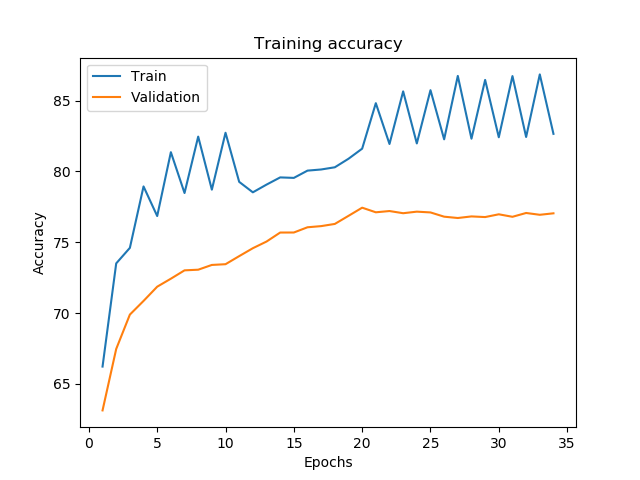
\includegraphics[width=\linewidth]{images/Model_general.png} % Figure image
	\caption{Historique d'entraînement} % Figure caption
	\label{histmodelnormal} 
\end{figure}


\subsection{Échantillonnage variable par classe}
La deuxième méthode d'entraînement est similaire à la première avec une légère modification qui essaie de privilégier les classes qui performment moins bien dans le but de simuler un processus de \emph{boosting}.


L'idée de base est d'échantillonner un plus grand nombre de données des classes qui sont mal prédites et un plus petit nombre pour celles qui sont bien prédites. À chaque epoch, on calcule notre accuracy par classe $A_i$ pour chacune des 340 classes. Pour effectuer notre epoch, on échantillonne $N_i$ données pour la classe i:

$$N_i=N(1-A_i)+0.25N$$
Où:
\begin{description}
\item[N]: Valeur constante pour toutes les classes (ex: 500)
\end{description}

Le terme $+0.25N$ permet de sélectionner au moins un minimum de données d'une classe qui perfomme déjà très bien pour que le modèle ne l'oublie pas lors la prochaine epoch.  Ainsi, on sélectionne $N$ données d'une classe avec 25\% d'accuracy et $0.35N$ données d'une classe qui a 90\% d'accuracy


En appliquant cette technique d'apprentissage, on obtient un accuracy de 79.53\% avec de l'early stopping.





\subsection{Modèle par ensemble avec couche de classification}
Le troisième modèle consiste à concaténer les sorties des 2 premiers modèles et les  passer dans une couche de classification linéaire. Pour l'entraînement de ce modèle, on gèle tous les paramètres des modèles \emph{Resnet18} et on entraîne seulement la couche de classification avec un échantillonnage fixe. La figure \ref{strutureensemble} illustre le processus.


\begin{figure}[h]
	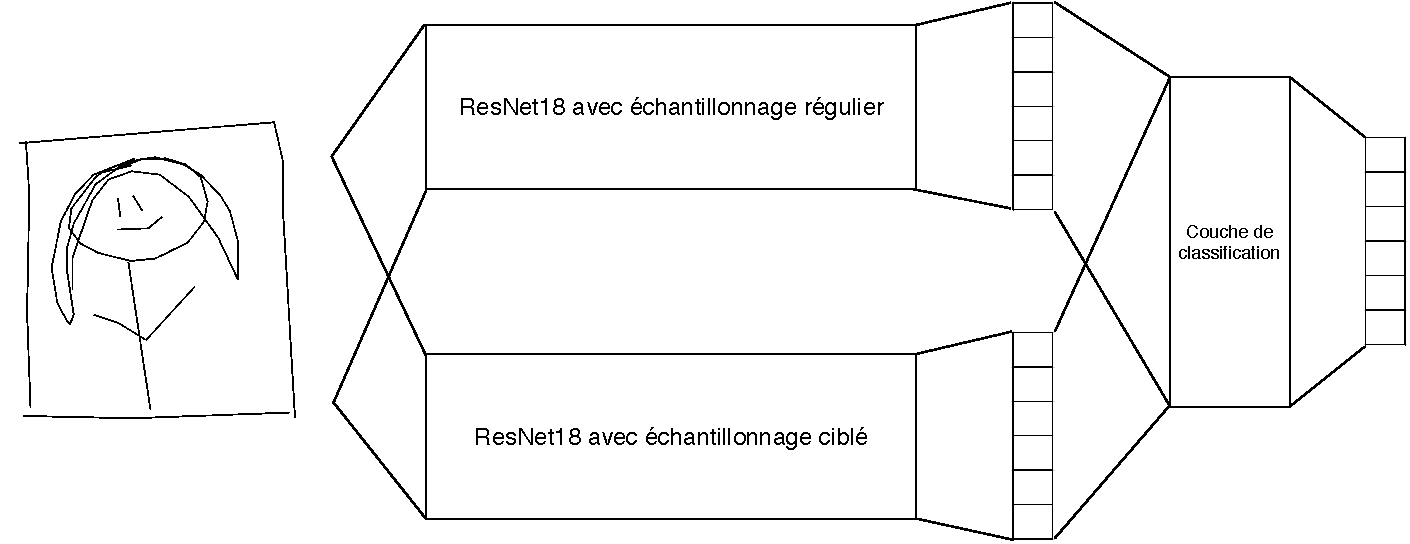
\includegraphics[width=\linewidth]{images/structure_reseau.pdf} % Figure image
	\caption{Modèle par ensemble avec couche de classification} % Figure caption
	\label{strutureensemble} 
\end{figure}


Par manque de temps, l'entraînement du modèle n'a pas pu être complété à 100\%, on peut toutefois voir l'historique d'entraînement du modèle sur la figure \ref{histmodelensemble}.


\begin{figure}[h]
	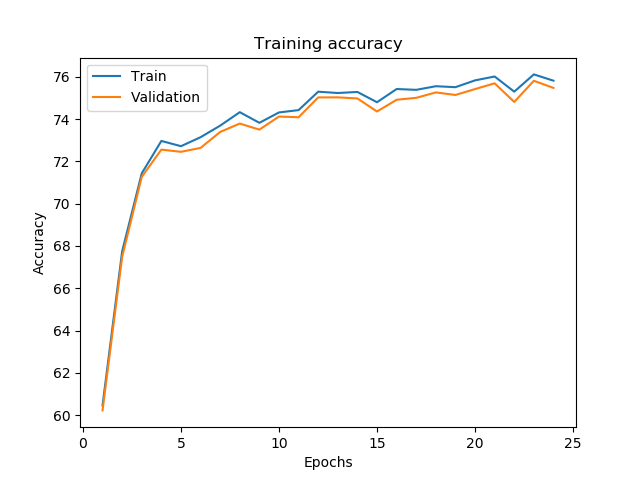
\includegraphics[width=\linewidth]{images/Model_ensemble.png} % Figure image
	\caption{Historique d'entraînement} % Figure caption
	\label{histmodelensemble} 
\end{figure}


On voit que l'accuracy sur le jeu d'entraînement est pratiquement identique à celle de validation et qu'elles ne semblent pas encore avoir atteint un plateau. Il aurait été intéressant de voir les résultats d'un plus grand nombre d'epochs. Avec un \emph{early stopping}, on obtient une accuracy de validation de 75.81\%. 


\subsection{Modèle par ensemble avec moyenne simple des 2 premiers modèles}

Le dernier modèle essayé consiste en une moyenne simple des 2 premiers modèles \emph{Resnet18}. Le modèle renvoie tout simplement la moyenne des deux sorties.
